%- - - - - - - - - - - - - - - - - - - - - - - - - - - - - - - - - SLIDE -
\frame{
\frametitle{ICPC}
\begin{block}{}
\begin{itemize}
	\item {\em International Collegiate Programming Contest}
	\item Competição de programação existente desde 1970 e organizada pela ACM desde 1977.
	\item Patrocinada pela IBM.
	\item A missão do ICPC é dar oportunidades aos estudantes para interagir com alunos de outras universidades e demonstrar sua capacidade de {\bf resolver problemas}, {\bf programar} e {\bf trabalhar em grupo}.
\end{itemize}
\end{block}
}

%- - - - - - - - - - - - - - - - - - - - - - - - - - - - - - - - - SLIDE -
\frame{
\frametitle{ICPC}
\begin{block}{}
\begin{itemize}
	\item A competição possui duas etapas
	\begin{itemize}
		\item Finais Regionais -- realizadas localmente, em vários países ao redor do mundo. 
		\item Final Mundial -- reúne os melhores colocados das competições regionais.
	\end{itemize}
	
	\item A etapa regional ocorre no ano anterior à final mundial
	\begin{itemize}
		\item Os times se classificam nas regionais de 2012 para competir a final mundial de 2013.
	\end{itemize}
	
	\item Apenas um time por instituição é classificado para a final mundial.
\end{itemize}
\end{block}
}

%- - - - - - - - - - - - - - - - - - - - - - - - - - - - - - - - - SLIDE -
\begin{frame}
\frametitle{ICPC}
\begin{center}
	\begin{minipage}{.9\textwidth}
	\centering
	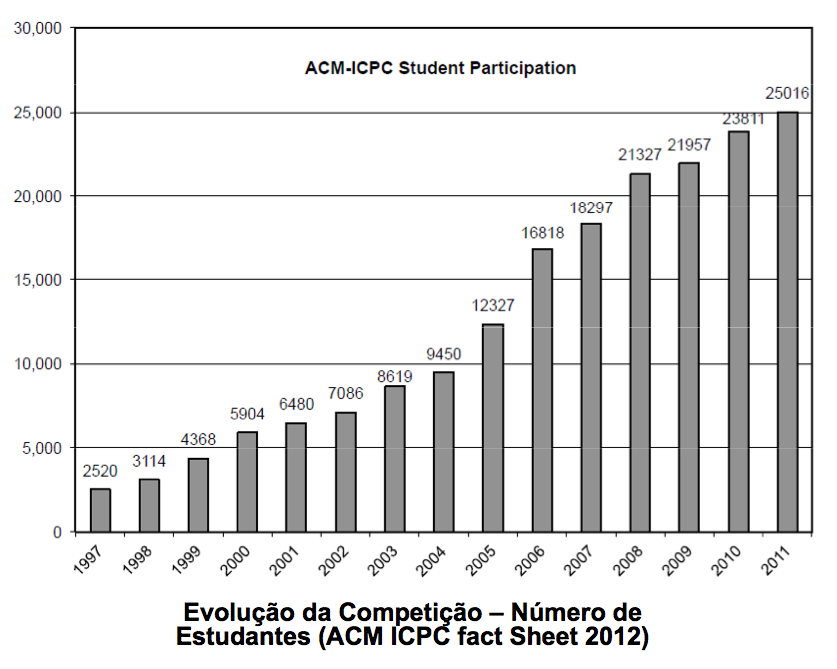
\includegraphics[width=.9\textwidth]{figuras/worldnmbrs.png}	
	\end{minipage}
\end{center}
\end{frame}

%- - - - - - - - - - - - - - - - - - - - - - - - - - - - - - - - - SLIDE -
\frame{
\frametitle{ICPC no mundo}
\begin{block}{}
\begin{itemize}
	\item 2007/2008: mais de 6700 times de 1821 escolas de 83 países.
	\begin{itemize}
		\item 100 participaram da Final Mundial do evento, em Banff, Canadá.
		\item Participação de 4 times brasileiros (IME, ITA, IME-USP, Unicamp) na final mundial.
	\end{itemize}

	\item 2011/2012: mais de 8338 times (mais de 25000 estudantes) de 2219 instituições de 88 países competiram em regionais nos 6 continentes.
	\begin{itemize}
		\item 112 times na Final Mundial do evento, em Varsóvia, Polônia.
		\item 6 times brasileiros (ITA,UFCG,UFPR,UFPE, UFRJ e IME-USP) participaram da final.
	\end{itemize}
\end{itemize}
\end{block}
}

%- - - - - - - - - - - - - - - - - - - - - - - - - - - - - - - - - SLIDE -
\begin{frame}
\frametitle{Maratona de Programação}
\begin{block}{ICPC no Brasil}
\begin{itemize}
	\item Maratona de Programação desde 1996.
	\item Realizada pela SBC desde o ano 2000.
	\item Apoio do CNPq desde 2002.
	\item Realizada em parceria com a Fundação Carlos Chagas desde o ano 2006.
\end{itemize}
\end{block}
\begin{center}
\begin{minipage}{.4\textwidth}
\frametitle{Maratona de Programação}
	\centering
	
\includegraphics[width=.75\textwidth]{logo/logomdp}
\end{minipage}
\end{center}
\end{frame}

%- - - - - - - - - - - - - - - - - - - - - - - - - - - - - - - - - SLIDE -
\begin{frame}
\frametitle{Maratona de Programação}
\begin{block}{Competição em duas fases}
\begin{description}[Sul Americana]
	\item [Regional] Classificatória para a final nacional.
	\item [Nacional] Final brasileira e classificatória para a final mundial.
\end{description}
\end{block}

\begin{block}{}
\small Na América do Sul existem três regionais do ICPC. 
\begin{itemize}
	\item \small South America/Brazil Regional -- A Final Nacional da Maratona de Programação.
	\item \small South America/North Regional -- Colômbia, Equador, Panamá, Venezuela.
	\item \small South America/South Regional -- Argentina, Bolívia, Chile, Peru, Paraguai, Uruguai.
\end{itemize}

\end{block}

\begin{block}{}
\begin{itemize}
	\item \url{http://maratona.ime.usp.br/}
	\item \url{http://www.inf.ufg.br/maratona/}
	\item \url{https://www.facebook.com/maratonago}
\end{itemize}
\end{block}
\end{frame}

%- - - - - - - - - - - - - - - - - - - - - - - - - - - - - - - - - SLIDE - 
\begin{frame}
\frametitle{Maratona de Programação}
\begin{center}
	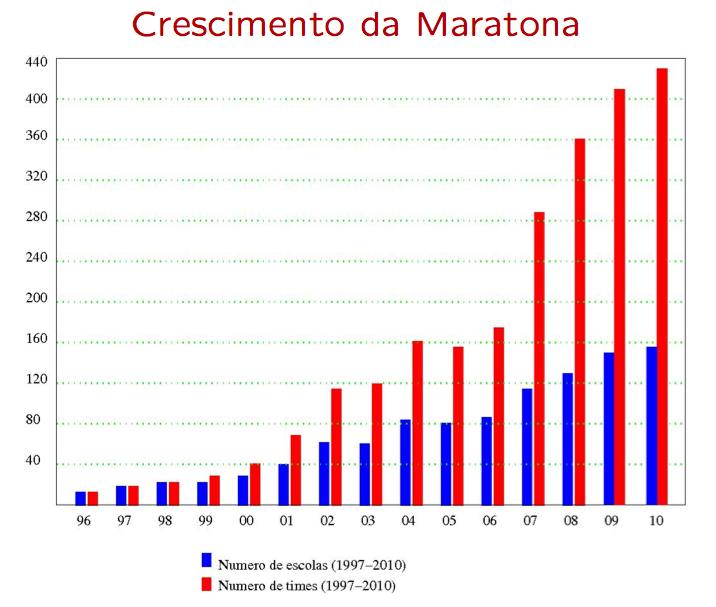
\includegraphics[width=.75\textwidth]{figuras/crescbrsl.png}
\end{center}
\end{frame}

%- - - - - - - - - - - - - - - - - - - - - - - - - - - - - - - - - SLIDE - 
\begin{frame}
\frametitle{Maratona de Programação}
\begin{center}
	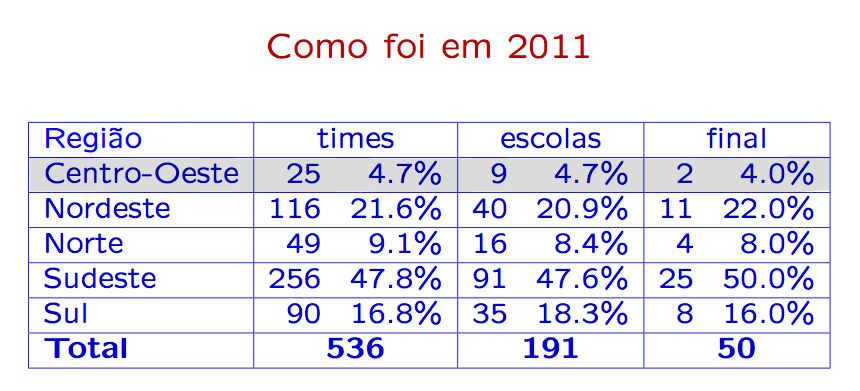
\includegraphics[width=.9\textwidth]{figuras/nmbrsl2.png}
\end{center}
\end{frame}

%- - - - - - - - - - - - - - - - - - - - - - - - - - - - - - - - - SLIDE -
\frame{
\frametitle{Maratona de Programação}
\begin{block}{Participação do INF - Fase Regional}
\centering
\begin{tabular}{ccccc}
\hline
{\bf Ano} & {\bf Local}       & {\bf Equipes} & {\bf Instituições} & {\bf Classificação} \\
\hline
2007     & Brasília-DF      & 5  & 3 & 3\textordmasculine \\
2008     & Goiânia-GO     & 7  & 3 & 1\textordmasculine\ e 3\textordmasculine \\
2009     & Goiânia-GO     & 11 & 4 &1\textordmasculine,3\textordmasculine\ e 4\textordmasculine \\
2010     & Goiânia-GO     & 10 & 3 &  1\textordmasculine, 4\textordmasculine, 6\textordmasculine\ e 8\textordmasculine \\
2011     & Goiânia-GO     & 14 & 4+1 & 1\textordmasculine, 2\textordmasculine, 5\textordmasculine\ e 8\textordmasculine \\
2012     & Goiânia-GO    & 10 & 3+1 & 1\textordmasculine, 2\textordmasculine, 3\textordmasculine\ , 6\textordmasculine\ e 8\textordmasculine \\
\hline
\end{tabular}
\end{block}
}

%- - - - - - - - - - - - - - - - - - - - - - - - - - - - - - - - - SLIDE -
\frame{
\frametitle{Maratona de Programação}
\begin{block}{Participação do INF - Final Brasileira}
\centering
\begin{tabular}{ccccc}
\hline
{\bf Ano} & {\bf Local}       & {\bf Equipes} & {\bf Instituições} & {\bf Classificação} \\
\hline
2008     & Vila Velha-ES & 51/360 & 129 & 28\textordmasculine\\
2009     & Campinas-SP & 52/410 & 145 & 22\textordmasculine\\ 
2010     & Joinville-SC & 51/432 & 157 & 20\textordmasculine\\
2011     & Goiânia-GO & 50/536 & 191 & 11\textordmasculine\\
2012     & Londrina-PR & 50/545 & 194 & 13\textordmasculine\\
\hline
\end{tabular}
\end{block}
}

%- - - - - - - - - - - - - - - - - - - - - - - - - - - - - - - - - SLIDE -
\begin{frame}
\frametitle{Maratona de Programação}
\begin{block}{Como funciona?}
\begin{itemize}
	\item Competição voltada para alunos de cursos de Ciência da Computação, Engenharia de Computação e áreas afins.
	\item Os times são compostos de três estudantes com até 5 anos de estudos universitários ou 23 anos de idade.
	\begin{itemize}
		\item Podem ter participado de no máximo 4 regionais e 1 final mundial.
	\end{itemize}
	\item Os times recebem de 8 a 12 problemas computacionais para serem resolvidos durante a competição (5 horas).
	\item Quando um time considera que resolveu um problema submete aos juízes que, {\em online}, dizem se a solução está ou não correta.
	\item Uma solução correta resolve um conjunto de testes dos juízes, desconhecido dos alunos e recebe um balão.
\end{itemize}
\end{block}
\end{frame}

%- - - - - - - - - - - - - - - - - - - - - - - - - - - - - - - - - SLIDE -
\begin{frame}
\frametitle{Maratona de Programação}
\begin{block}{Como funciona?}
\begin{itemize}
	\item Você deve saber programar em C, C++ ou Java.
	\item Cada equipe tem acesso a um computador, sem conexão à internet, e apenas a material impresso.
	\item Objetivo é apresentar soluções computacionalmente corretas para um dado problema no menor tempo possível.
	\begin{itemize}
		\item O time vencedor é aquele que resolver mais problemas durante as 5 horas de competição
		\item Em caso de empate vence o time com a menor ``penalidade''
		\begin{itemize}
			\item Soma das penalidades dos problemas corretamente resolvidos;
			\item A penalidade de um problema é dada pelo número de minutos decorridos desde o início da competição até o momento da primeira submissão correta;
			\item Uma penalidade de 20 minutos é adicionada por cada submissão incorreta feita antes da primeira submissão correta.
		\end{itemize}
   	\end{itemize}
\end{itemize}
\end{block}
\end{frame}

%- - - - - - - - - - - - - - - - - - - - - - - - - - - - - - - - - SLIDE -
\begin{frame}
\frametitle{Maratona de Programação}
\begin{block}{Como funciona?}
\begin{itemize}
	\item Cada problema contém:
	\begin{itemize}
		\item Informações para contextualização (Background)
		\item O enunciado do problema
		\item Informações sobre a entrada (Input)
		\item Informações sobre a saída (Output)
		\item Exemplo de entrada (Sample Input)
		\item Exemplo de saída (Sample Output)
	\end{itemize}
\end{itemize}
\end{block}
\end{frame}

%- - - - - - - - - - - - - - - - - - - - - - - - - - - - - - - - - SLIDE -
\begin{frame}
\frametitle{Maratona de Programação}
\begin{block}{Como funciona?}
\begin{itemize}
	\item Os juízes possuem datasets que são utilizados para testar a solução submetida
	\item Esses datasets contém instâncias de testes bastante diferentes dos exemplos contidos nos problemas do caderno de questões
	\item Os juízes informarão uma das seguintes respostas a uma solução submetida por um time (sem nenhum detalhe adicional)
	\begin{itemize}
		\item Yes
		\item No - Wrong Answer (WA)
		\item No - Presentation Error (PE)
		\item No - Time Limit Exceeded (TLE)
		\item No - Runtime Error (RE)
		\item No - Compile Error (CE)
	\end{itemize}
	\item O sistema não responde nada além disto. Não é possível saber, por exemplo, se um programa que recebeu TLE produz a saída correta, ou em qual linha está o erro de um programa que recebeu CE.

\end{itemize}
\end{block}
\end{frame}

%- - - - - - - - - - - - - - - - - - - - - - - - - - - - - - - - - SLIDE -
\begin{frame}
\frametitle{Maratona de Programação}
\begin{block}{E se eu me der bem?}
\begin{itemize}
	\item Os melhores colocados da primeira fase por sede avançam para a Final Nacional da Maratona de Programação.
	\item Medalhas aos 10 primeiros colocados na final nacional
	\begin{itemize}
		\item Ouro para os três primeiros
		\item Prata para os três seguintes
		\item Bronze para os quatro últimos
	\end{itemize}
	\item Cópia do Troféu ``Maratona de Programação'' para o vencedor
	\item Premiação para os melhores colocados de cada região
	\item Vencedor ganha vaga na Final Mundial do ICPC
	\begin{itemize}
		\item Outros \em{N} times melhores colocados podem ter direito a participar da Final Mundial, dependendo do nro. de vagas adicionais atribuídas ao Brasil.
	\end{itemize}
\end{itemize}
\end{block}
\end{frame}

%- - - - - - - - - - - - - - - - - - - - - - - - - - - - - - - - - SLIDE -
%\begin{frame}
%\frametitle{Maratona de Programação}
%\begin{block}{Objetivos}
%\begin{itemize}
%	\item Atrair o maior número de estudantes.
%	\item Atrair o maior número de escolas.
%	\item Envolver o maior número de países.
%	\item Prover condições iguais aos times para chegar às finais mundiais.
%	\item Criar competições disputadas.
%	\item Valorizar os estudantes e os voluntários.
%\end{itemize}
%\end{block}
%\end{frame}